\documentclass[11pt, aspectratio=169]{beamer}
\usetheme{Madrid}
\usecolortheme{whale}

% --- Packages ---
\usepackage{graphicx}
\usepackage{booktabs}
\usepackage{multicol}
\usepackage{hyperref}
\usepackage{tabularx}
\usepackage{array}

% --- Meta Data ---
\title[POSETTE 2026]{Modelling Postgres Performance Degradation}
\subtitle{on Burstable Cloud Instances}
\author[Goh Chun Lin]{Goh Chun Lin}
\institute[.NET Foundation]{.NET Foundation Member}
\date[June 18, 2026]{June 18, 2026}

\begin{document}

% --- Slide 1: Title Slide ---
\begin{frame}[plain]
    \titlepage
\end{frame}

% --- Slide 2: The Appeal of Burstable Instances ---
\begin{frame}{The Appeal of Burstable Instances}
    \begin{block}{Cost-Effective Cloud Computing}
        \begin{itemize}
            \item Azure B-series (Burstable PostgreSQL)
            \item Similar offerings: AWS T-series, GCP E2 (burstable)
            \item 20--60\% cheaper than fixed-performance instances
        \end{itemize}
    \end{block}

    \vfill
    \begin{alertblock}{The Core Question}
        Perfect for variable workloads\dots right?
    \end{alertblock}
\end{frame}

% --- Slide 3: Token Bucket Algorithm ---
\begin{frame}{Token Bucket Algorithm}
    \begin{center}
        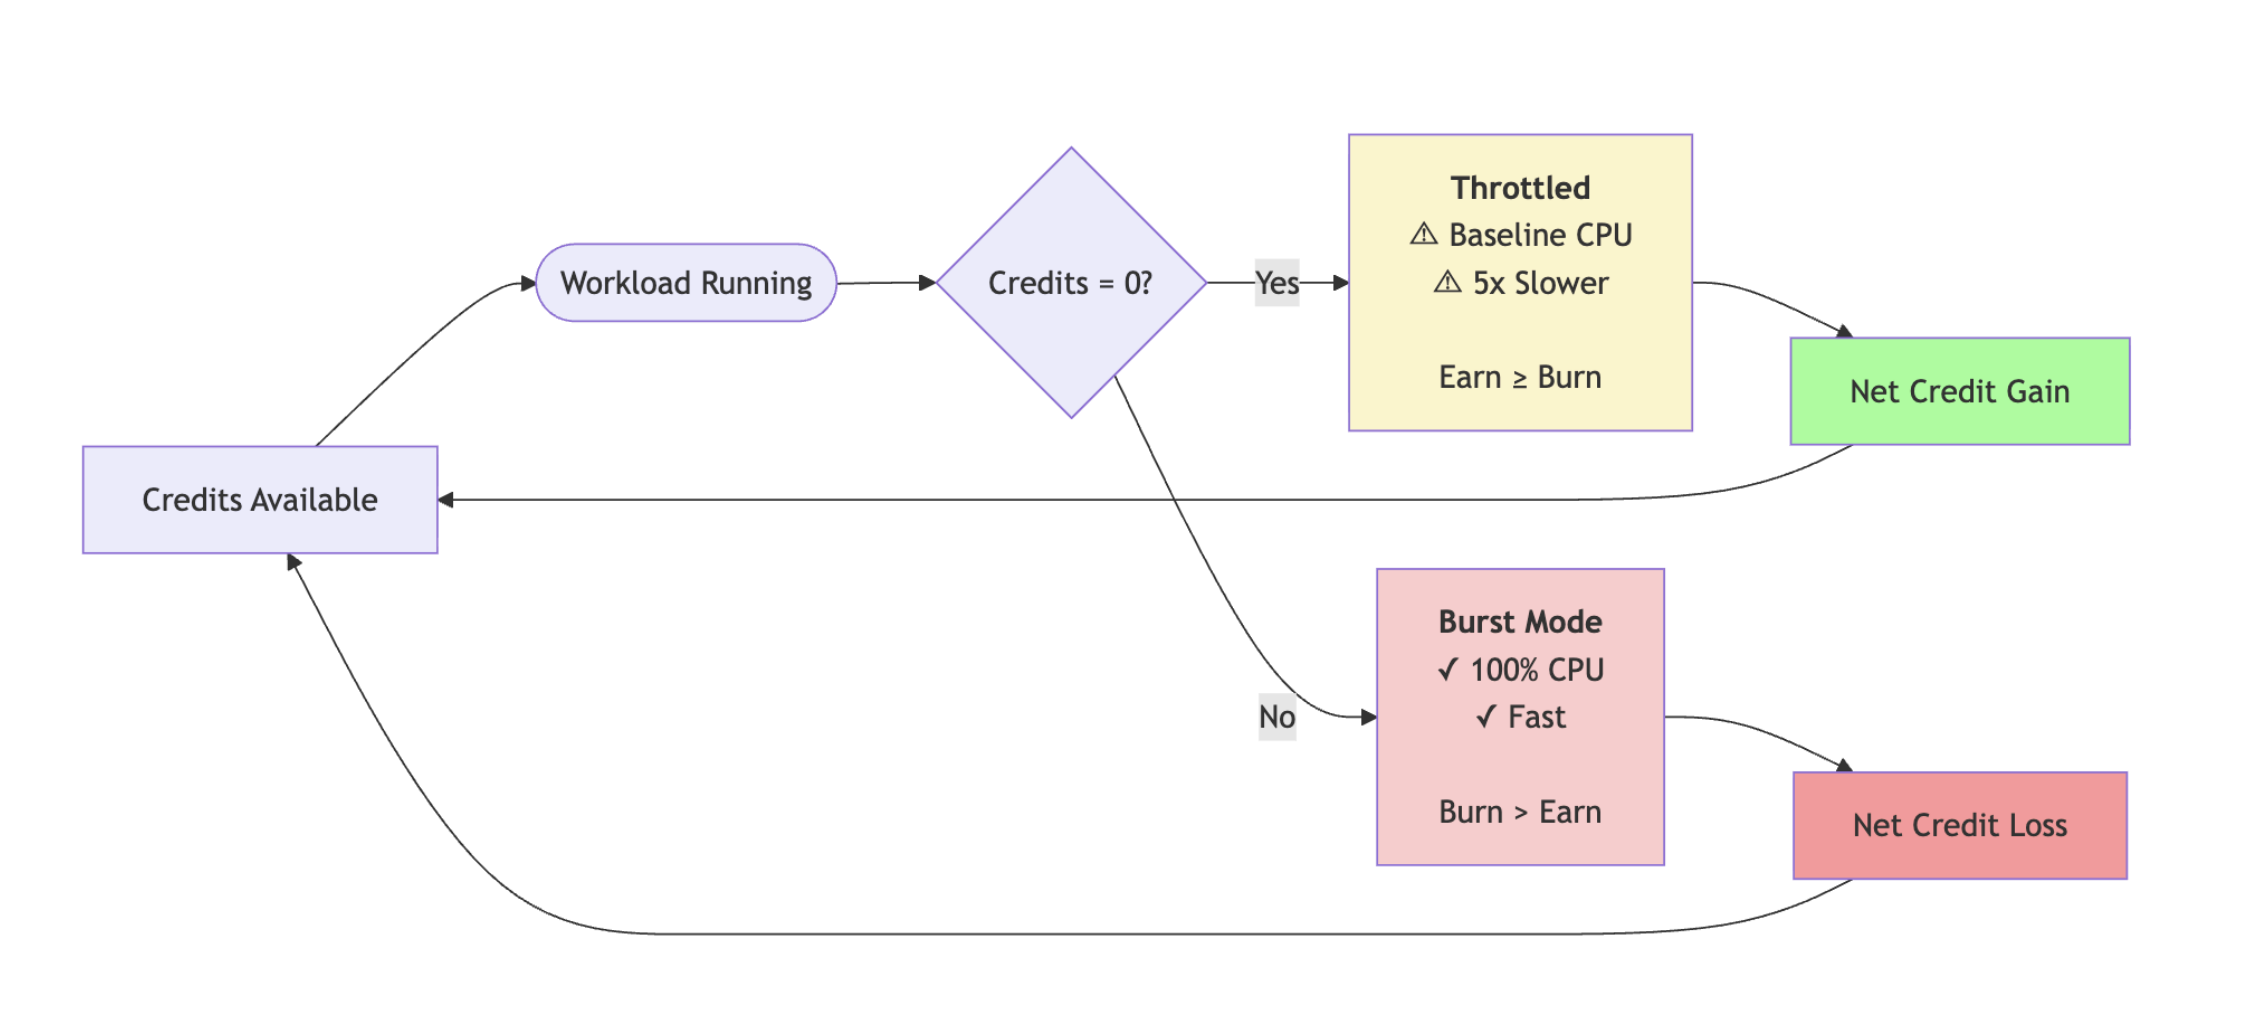
\includegraphics[width=\textwidth]{images/token-bucket-algorithm.png}
    \end{center}
    % SPEAKER NOTES:
    % flowchart LR
    %   Credits[Credits Available] --> Query([Workload Running])
    %
    %   Query --> Check{Credits = 0?}
    %
    %   Check -->|Yes| Throttle[<b>Throttled</b><br/>⚠ Baseline CPU<br/>⚠ 5x Slower<br/><br/>Earn ≥ Burn]
    %   Check -->|No| Burst[<b>Burst Mode</b><br/>✓ 100% CPU<br/>✓ Fast<br/><br/>Burn > Earn]
    %
    %   Burst --> NetBurn[Net Credit Loss]
    %   Throttle --> NetGain[Net Credit Gain]
    %
    %   NetBurn --> Credits
    %   NetGain --> Credits
    %
    %   style Burst fill:#ffcccc
    %   style Throttle fill:#fff4cc
    %   style NetBurn fill:#ff9999
    %   style NetGain fill:#99ff99
\end{frame}

% --- Slide 4: The CPU Credit Model ---
\begin{frame}{The CPU Credit Model}
    \textbf{How it works:}
    \begin{enumerate}
        \item Earn credits continuously over time
        \item Burn credits when using CPU above baseline
        \item Burst to 100\% CPU when credits available
        \item Throttle to baseline when depleted
    \end{enumerate}

    \vfill
    \begin{exampleblock}{Example Blueprint: Azure B2ms}
        \begin{itemize}
            \item Base CPU Performance of VM: 30\%
            \item Earns 36 credits/hour, burns 2 credits/min at burst
        \end{itemize}
    \end{exampleblock}
\end{frame}

% --- Slide 5: Azure B-series V1 CPU Burst ---
\begin{frame}{Azure B-series V1 CPU Burst}
    \begin{columns}[c]
        \begin{column}{0.65\textwidth}
            \begin{center}
                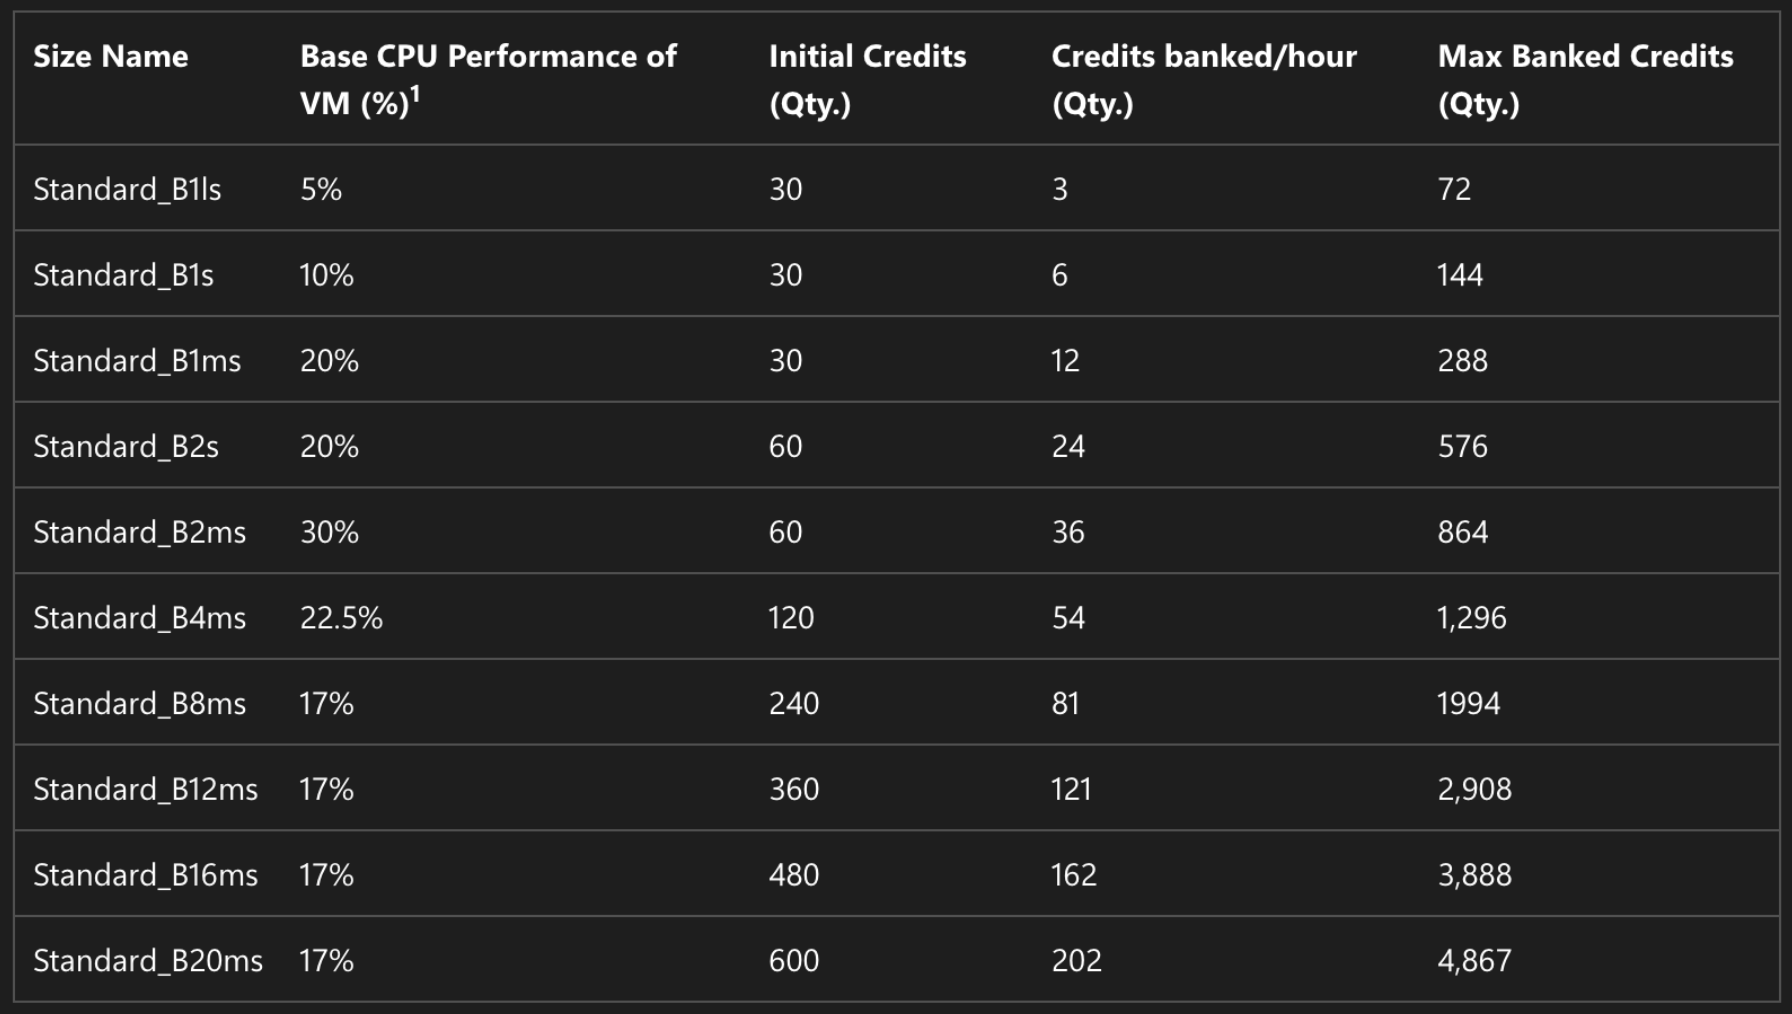
\includegraphics[width=\textwidth]{images/azure-cpu-table.png}
            \end{center}
        \end{column}
        
        \begin{column}{0.3\textwidth}
            \begin{center}
                Reference Documentation:\\[0.5em]
                
\includegraphics[width=0.8\textwidth]{images/azure-cpu-table-qrcode.png}
            \end{center}
        \end{column}
    \end{columns}
\end{frame}

% --- Slide 6: The Hidden Danger ---
\begin{frame}{The Hidden Danger}
    \textbf{Not a crash. Not an error. Just\dots slowness.}
    \vfill
    When CPU credits deplete:
    \begin{itemize}
        \item Database throttles to baseline CPU;
        \item Query time increases significantly (5x minimum, often worse);
        \item Postgres does not know it's being throttled;
        \item Slow queries hold connections longer.
    \end{itemize}
    \vfill
    \begin{alertblock}{Result}
        Connection pool exhaustion.
    \end{alertblock}
\end{frame}

% --- Slide 7: The Cascading Failure ---
\begin{frame}{The Cascading Failure}
    \textbf{Watch how one problem triggers the next:} 
    \vfill
    When connections held longer:
    \begin{itemize}
        \item Connection pool saturates;
        \item New requests queue;
        \item P99 latency spikes and app layer times out;
        \item max\_connections limit hit;
        \item PostgreSQL rejects connections.
    \end{itemize}
    \vfill
    \begin{alertblock}{Result}
        At this point, you are experiencing a severe production outage.
    \end{alertblock}
\end{frame}

% --- Slide 8: The Restart Loop ---
\begin{frame}{The Restart Loop}
    \textbf{But wait - it gets worse:}
    \vfill
    When PostgreSQL rejects connection:
    \begin{itemize}
        \item Health checks fail;
        \item Orchestrator on Azure restarts the database;
        \item Boot sequence burns remaining CPU credits;
        \item Comes back up already slow and immediately saturates again;
        \item Manual intervention required to break the loop.
    \end{itemize}
\end{frame}

% --- Slide 9: The Challenge: Incomplete Information ---
\begin{frame}{The Challenge: Incomplete Information}
    \textbf{You can calculate credit rates. You can monitor credit balance.}
    \textbf{But predicting interactions requires testing.}
    \vfill
    \begin{center}
        \newcolumntype{Y}{>{\raggedright\arraybackslash}X}

        \begin{tabularx}{\textwidth}{YYY}
            \toprule
            \textbf{Over-provision} & \textbf{Load test all configs} & \textbf{Simulate} \\
            \midrule
            Skip the B-series entirely and pay for General Purpose. & Trial by fire. Test every possible configuration. & Use the math to model the traffic. Test 50 scenarios in hours. \\[0.8em]
            
            {\small\color{green!60!black}$\checkmark$ Safe} & 
            {\small\color{green!60!black}$\checkmark$ Accurate} & 
            {\small\color{green!60!black}$\checkmark$ Good enough} \\[0.5em]
            
            {\small\color{red!80!black}$\times$ Expensive at scale} & 
            {\small\color{red!80!black}$\times$ Weeks of work} & 
            {\small\color{green!60!black}$\checkmark$ Fast} \\
            \bottomrule
        \end{tabularx}
    \end{center}
\end{frame}

% --- Slide 10: Simulation Approach ---
\begin{frame}{Simulation Approach}
    \textbf{Models credit mechanics, pooling modes, and queueing behavior}
    \vfill
    \textbf{Simulation is a filter, not a total replacement for reality.}
    \begin{itemize}
        \item Reduces load testing scope (test 3 finalists, not 50 configs)
    \end{itemize}
    \vfill
    \textbf{Simulation finds candidates. Load testing validates the finalists.}
\end{frame}

% --- Slide 11: Why Discrete Event Simulation (DES)? ---
\begin{frame}{Why Discrete Event Simulation (DES)?}
    \begin{block}{Definition}
        \textbf{DES:} Models systems by following each event step by step.
    \end{block}

    \vfill
    \textbf{DES models pooling, CPU credits, queueing in burstable instances.}
\end{frame}

% --- Slide 12: Modelling as Discrete Event Simulation ---
\begin{frame}{Modelling as Discrete Event Simulation}
    \textbf{Burstable instances are not magic. They follow a strict mathematical model called the Token Bucket Algorithm.}
    \vfill
    \begin{columns}[t]
        \begin{column}{0.3\textwidth}
            \begin{block}{Generator}
                \begin{center}
                    {\small Load Generator}
                \end{center}
            \end{block}
        \end{column}
        \begin{column}{0.3\textwidth}
            \begin{block}{Queue}
                \begin{center}
                    {\small DB Connection Pool}
                \end{center}
            \end{block}
        \end{column}
        \begin{column}{0.3\textwidth}
            \begin{block}{Server}
                \begin{center}
                    {\small Burstable Instance}
                \end{center}
            \end{block}
        \end{column}
    \end{columns}
\end{frame}

% --- Slide 13: What is SNA? ---
\begin{frame}{What is SNA?}
    \begin{columns}[c]
        \begin{column}{0.65\textwidth}
            A lightweight open-source library for Discrete Event Simulations in C\# and .NET 10.
            
            \vspace{1em}
            \textbf{Available to model Azure Database for PostgreSQL B-series with M/M/c/K:}
            \begin{itemize}
                \item Deterministic logic for stochastic inputs;
                \item Configurable baseline/earn rates (adapts to any B-series specs);
                \item Validated against queueing theory predictions.
            \end{itemize}
        \end{column}
        
        \begin{column}{0.3\textwidth}
            \begin{center}
                Project repo:\\[0.5em]
                
\includegraphics[width=0.8\textwidth]{images/sna-github-qrcode.png}
            \end{center}
        \end{column}
    \end{columns}
\end{frame}

% --- Slide 14: CPU Credits Simulation (Transition Slide) ---
\begin{frame}
    \begin{center}
        \Large\textbf{CPU Credits Simulation}
        \vspace{1.5em}
        
        \color{blue}\textbf{Question:}\\
        \large\color{black}Where is the point where specific workload transitions from "Bursting" to "Death Spiral"?
    \end{center}
\end{frame}

% --- Slide 15: Credit Mechanics ---
\begin{frame}{Credit Mechanics}
    \begin{center}
        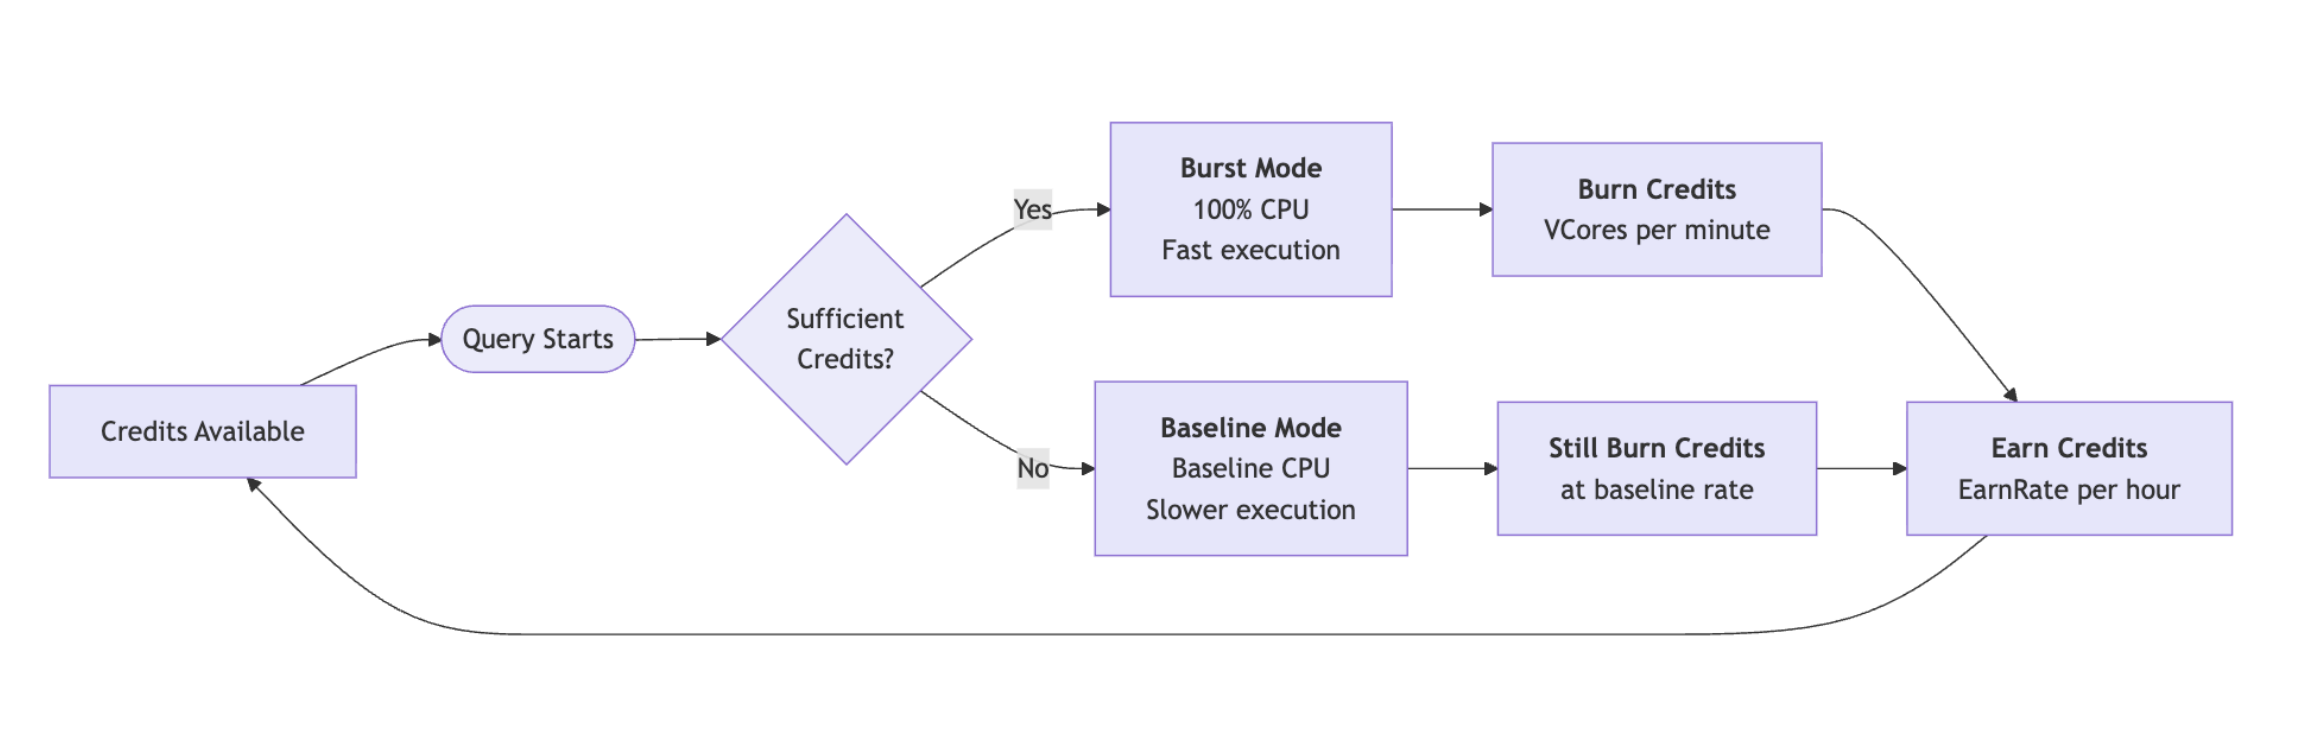
\includegraphics[width=\textwidth]{images/demo3.1.png}
    \end{center}
    % SPEAKER NOTES:
    % flowchart LR
    %   Credits[Credits Available] --> Query([Query Starts])
    %   
    %   Query --> Check{Sufficient<br/>Credits?}
    %   
    %   Check -->|Yes| Burst[<b>Burst Mode</b><br/>100% CPU<br/>Fast execution]
    %   Check -->|No| Baseline[<b>Baseline Mode</b><br/>Baseline CPU<br/>Slower execution]
    %   
    %   Burst --> BurnFast[<b>Burn Credits</b><br/>VCores per minute]
    %   Baseline --> BurnSlow[<b>Still Burn Credits</b><br/>at baseline rate]
    %   
    %   BurnFast --> Earn[<b>Earn Credits</b><br/>EarnRate per hour]
    %   BurnSlow --> Earn
    %   
    %   Earn --> Credits
    %   
    %   style Burst fill:#e6e6ff
    %   style Baseline fill:#e6e6ff
    %   style BurnFast fill:#e6e6ff
    %   style BurnSlow fill:#e6e6ff
    %   style Earn fill:#e6e6ff
    %   style Credits fill:#e6e6ff
\end{frame}

% --- Slide 16: Credit Depletion Timeline ---
\begin{frame}{Credit Depletion Timeline}
    \begin{columns}[c]
        \begin{column}{0.45\textwidth}
            \textbf{What we're seeing:}
            \begin{itemize}
                \item Credits start at 60;
                \item Linear depletion as burst usage exceeds earn rate;
                \item Credits hit zero at ~1,300 seconds;
                \item \textbf{This is your burst tolerance window: $\sim$20 minutes.}
            \end{itemize}
            \vspace{1em}
            \textit{\small *Note: Starting credits affect timeline. Tune this parameter to match your environment.}
        \end{column}
        
        \begin{column}{0.5\textwidth}
            \begin{center}
                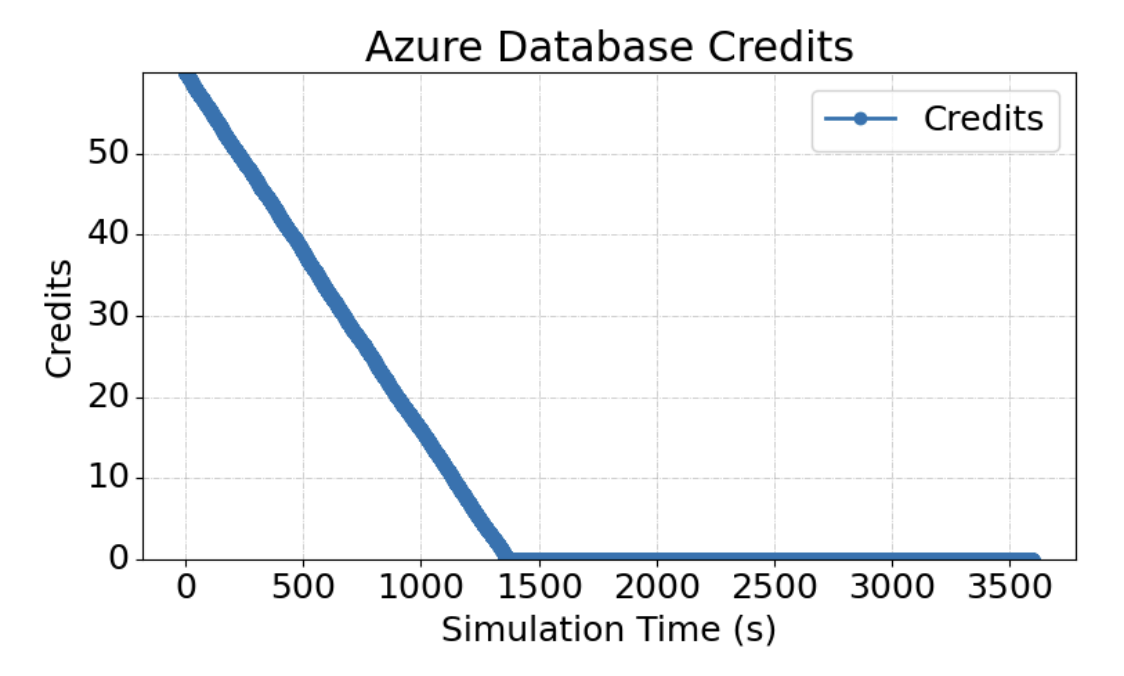
\includegraphics[width=\textwidth]{images/simulation_credits.png}
            \end{center}
        \end{column}
    \end{columns}
\end{frame}

% --- Slide 17: The Performance Cliff ---
\begin{frame}{The Performance Cliff}
    \begin{columns}[c]
        \begin{column}{0.45\textwidth}
            \textbf{What happens when credits hit zero:}
            \begin{itemize}
                \item Simulation shows 5x degradation for CPU-bound queries;
                \item Production cascading effects often worse.
            \end{itemize}
            \vfill
            \begin{alertblock}{Takeaway}
                This is why "database is up" does not mean database is working.
            \end{alertblock}
        \end{column}
        
        \begin{column}{0.5\textwidth}
            \begin{center}
                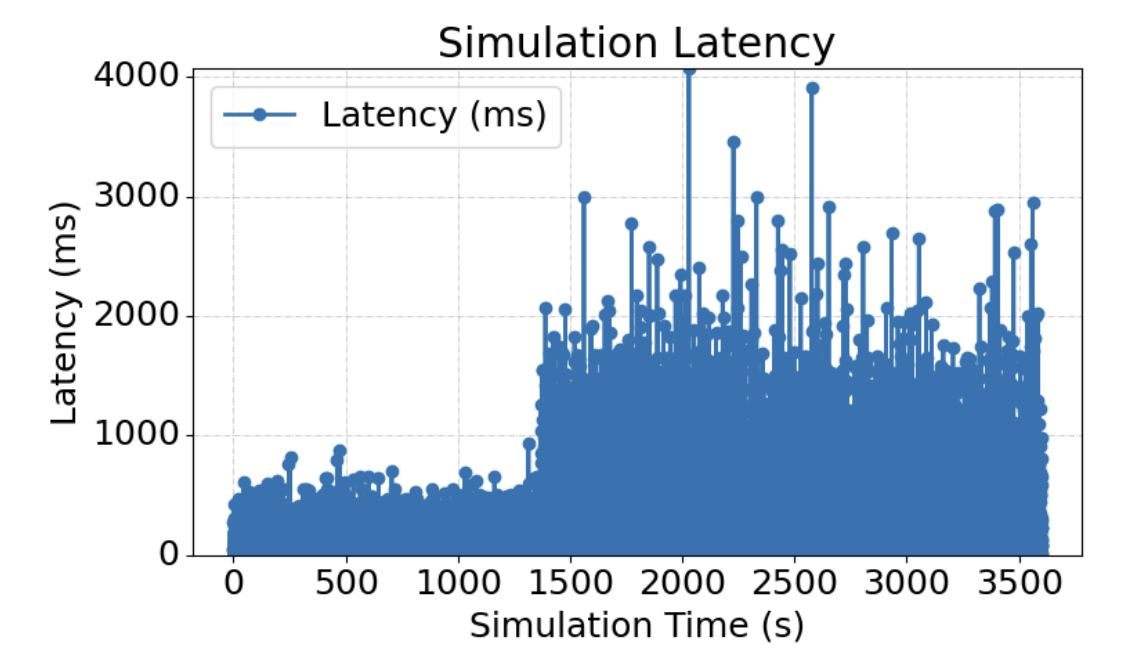
\includegraphics[width=\textwidth]{images/simulation_latency.png}
            \end{center}
        \end{column}
    \end{columns}
\end{frame}

% --- Slide 18: Demo 2: Pool Size Optimization (Transition Slide) ---
\begin{frame}
    \begin{center}
        \Large\textbf{Demo 2: Pool Size Optimization}
        \vspace{1.5em}
        
        \color{blue}\textbf{Question:}\\
        \large\color{black}How big should my connection pool be?
    \end{center}
\end{frame}

% --- Slide 19: Demo 2: Testing Pool Sizes ---
\begin{frame}{Demo 2: Testing Pool Sizes}
    \textbf{Testing common assumptions:}
    \vfill
    \begin{center}
        \begin{tabular}{ll}
            \toprule
            \textbf{Pool Size} & \textbf{Common Industry Rationale} \\
            \midrule
            5 & "Too small?" \\
            10 & "Rule of thumb: use 10" \\
            20 & "2x CPU cores (B2ms has 2 vCPU)" \\
            50, 100 & "Just set it high to be safe" \\
            \bottomrule
        \end{tabular}
    \end{center}
    \vfill
    \textbf{Parameters:} Session pooling configuration, 50 requests/sec continuous steady-state load.\\
    \textbf{Objective:} Isolate the minimum pool footprint within 5\% of optimal latency.
\end{frame}

% --- Slide 20: Demo 2: Results ---
\begin{frame}{Demo 2: Results}
    \begin{columns}[c]
        \begin{column}{0.45\textwidth}
            \textbf{Key findings:}
            \begin{itemize}
                \item \textbf{Pool Size 5:} $\sim$67ms (queueing visible)
                \item \textbf{Pool Size 10:} $\sim$57ms (optimal for steady load)
                \item \textbf{Pool Size 20--100:} $\sim$56ms (no latency gain, but handles micro-bursts)
            \end{itemize}
        \end{column}
        
        \begin{column}{0.5\textwidth}
            \begin{center}
                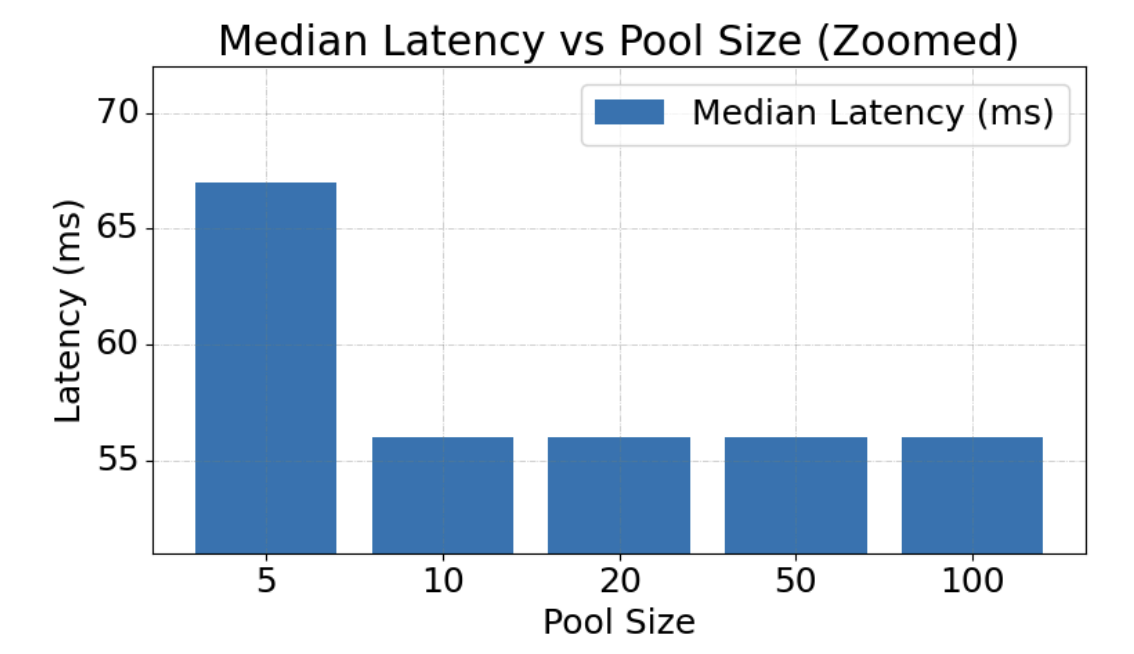
\includegraphics[width=\textwidth]{images/latency_bar_chart_zoomed.png}
            \end{center}
        \end{column}
    \end{columns}
\end{frame}

% --- Slide 21: Cross-Cloud Applicability ---
\begin{frame}{Cross-Cloud Applicability}
    \textbf{Industry-standard credit model:}
    \begin{itemize}
        \item \textbf{Azure B-series}, AWS T-series, GCP E2, Oracle burstable
        \item All use: earn credits -> burn when bursting -> throttle when depleted
    \end{itemize}

    \vfill
    \textbf{Minor differences:} Initial credits, unlimited mode, baseline \%
    \vfill
    \textbf{Same approach works across all cloud providers.}
\end{frame}

% --- Slide 22: When Simulation Is Worth It ---
\begin{frame}{When Simulation Is Worth It}
    \textbf{Startup (10 instances):} Just guess (config changes are fast) \\
    \textbf{Enterprise (50+ instances):} Simulate (saves \$50k/year vs over-provisioning)
    \vfill
    \textbf{This model covers:} CPU credits, connection pooling, queueing \\
    \textbf{Does not model:} IOPS throttling, network throttling, storage latency
\end{frame}

% --- Slide 23: One More Thing: Observability (Transition Slide) ---
\begin{frame}
    \begin{center}
        \Large\textbf{One More Thing}
        \vspace{1.5em}
        
        \large\color{blue}Observability
    \end{center}
\end{frame}

% --- Slide 24: Observability: OpenTelemetry Integration ---
\begin{frame}{Observability: OpenTelemetry Integration}
    \begin{columns}[c]
        \begin{column}{0.5\textwidth}
            \begin{center}
                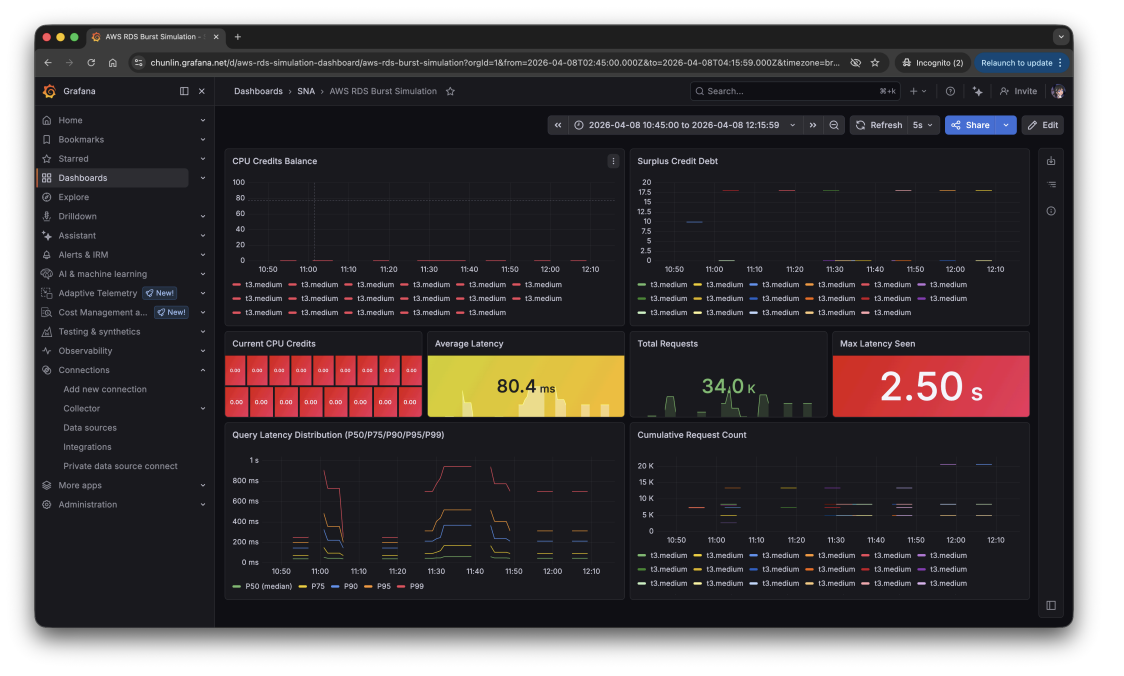
\includegraphics[width=\textwidth]{images/grafana-dashboard.png}
            \end{center}
        \end{column}
        
        \begin{column}{0.45\textwidth}
            \textbf{What you're seeing:}
            \begin{itemize}
                \item \textbf{Credits depleted:} All instances at 0.00 (red boxes)
                \item \textbf{Performance cliff:} Max latency exploded to 2.5 seconds
                \item \textbf{The problem made visible:} Average 80ms looks fine, but p99 catastrophic
            \end{itemize}
            \vfill
            \textbf{SNA exports OpenTelemetry metrics for real-time monitoring}
        \end{column}
    \end{columns}
\end{frame}

% --- Slide 25: From Guessing to Knowing ---
\begin{frame}{From Guessing to Knowing}
    \begin{tabular}{ll}
        \toprule
        \textbf{Before Simulation} & \textbf{After Simulation} \\
        \midrule
        Guess pool size & Calculated optimal size \\
        Test in production & Test in simulation first \\
        Risk of downtime & Identified failure points \\
        Days to tune & 1 minute to narrow options \\
        Over-provision 2-5x & Data-driven right-sizing \\
        \bottomrule
    \end{tabular}
\end{frame}

% --- Slide 26: Thank You ---
\begin{frame}
    \begin{center}
        \textbf{Thank You}
        \vspace{2em}
        
        \textbf{GitHub Repository:} \\
        \href{https://github.com/gcl-team/SNA}{github.com/gcl-team/SNA}
        
        \vspace{1em}
        \textbf{Contact:} \\
        Goh Chun Lin \\
        \href{https://www.linkedin.com/in/gohchunlin}{linkedin.com/in/gohchunlin}
    \end{center}
\end{frame}

\end{document}